\section{Diffusion-Reaction Equation With Nernst Convection Term.}


The complete dynamic system is given by

\begin{align} \label{eq:diffusion-nernst}
\frac{\partial C_+}{\partial t} &= \mathcal{D_+}\left(\nabla^2 C_+(x) +\nabla \cdot \qty{C_+(x)\qty{\frac{z \mathcal{F}}{RT}\nabla\phi(x)}}\right), \\
\frac{\partial C_-}{\partial t} &= \mathcal{D_-}\left(\nabla^2 C_-(x) -\nabla \cdot \qty{C_-(x)\qty{\frac{z \mathcal{F}}{RT}\nabla\phi(x)}}\right),\\
	\nabla^2 \phi &= \frac{\qty{z\mathcal{F}}}{\epsilon}\qty{C_- - C_+}.
\end{align}

Boundary conditions are fixed by the flux at the interface and boundary conditions at the bulk.

\begin{align}
    J_+(x = 0) &= -\mathcal{D}_+\qty{\frac{\partial C_+}{\partial x} - C_+ \frac{z\mathcal{F}}{RT}\frac{\partial\phi}{\partial x}}\bigg|_{x= 0}= -k_f C_+(x = 0, t),\\
    J_-(x = 0) &= -\mathcal{D}_-\qty{\frac{\partial C_-}{\partial x} + C_- \frac{z\mathcal{F}}{RT}\nabla\phi} \bigg|_{x= 0} = 0,\\
    C_+(\delta) = C_b,\\
    C_-(\delta) = C_b,\\
    \phi(x = 0) &= V_0,\\
    \phi(x = \delta) &= 0.
\end{align}

Initial conditions are given by

\begin{align}
	C_s(x, t=0) = 0,\\
	\phi (x,t=0) = 0.
\end{align}

Let 

\begin{align}
	\Psi(x, t) = \frac{z\mathcal{F}}{RT}\phi(x, t), \\
	\rho_s(x, t) = \frac{C_s(x, t)}{C_b},
\end{align}

be the adimentional potential and adimentional concentration where $s=\pm$ and 

\begin{align}
	\label{eq:ionic-force}
	\kappa = \sqrt{\frac{\qty{z\mathcal{F}}^2C_b}{\epsilon RT}}.
\end{align}

be the ionic force.

In Appendix \ref{appendix:analytic-diff-only} the numerical algorithm generalized from previous section from diffusion type problems into Nernst-Planck type problem is outlined. Figure \ref{fig:nernst-planck} shows results for the electric potential as an example. In chapter \ref{ch:results-analysis} further results are shown, derived from the results obtained with this algorithm.

\begin{figure}[htbp]
\centering
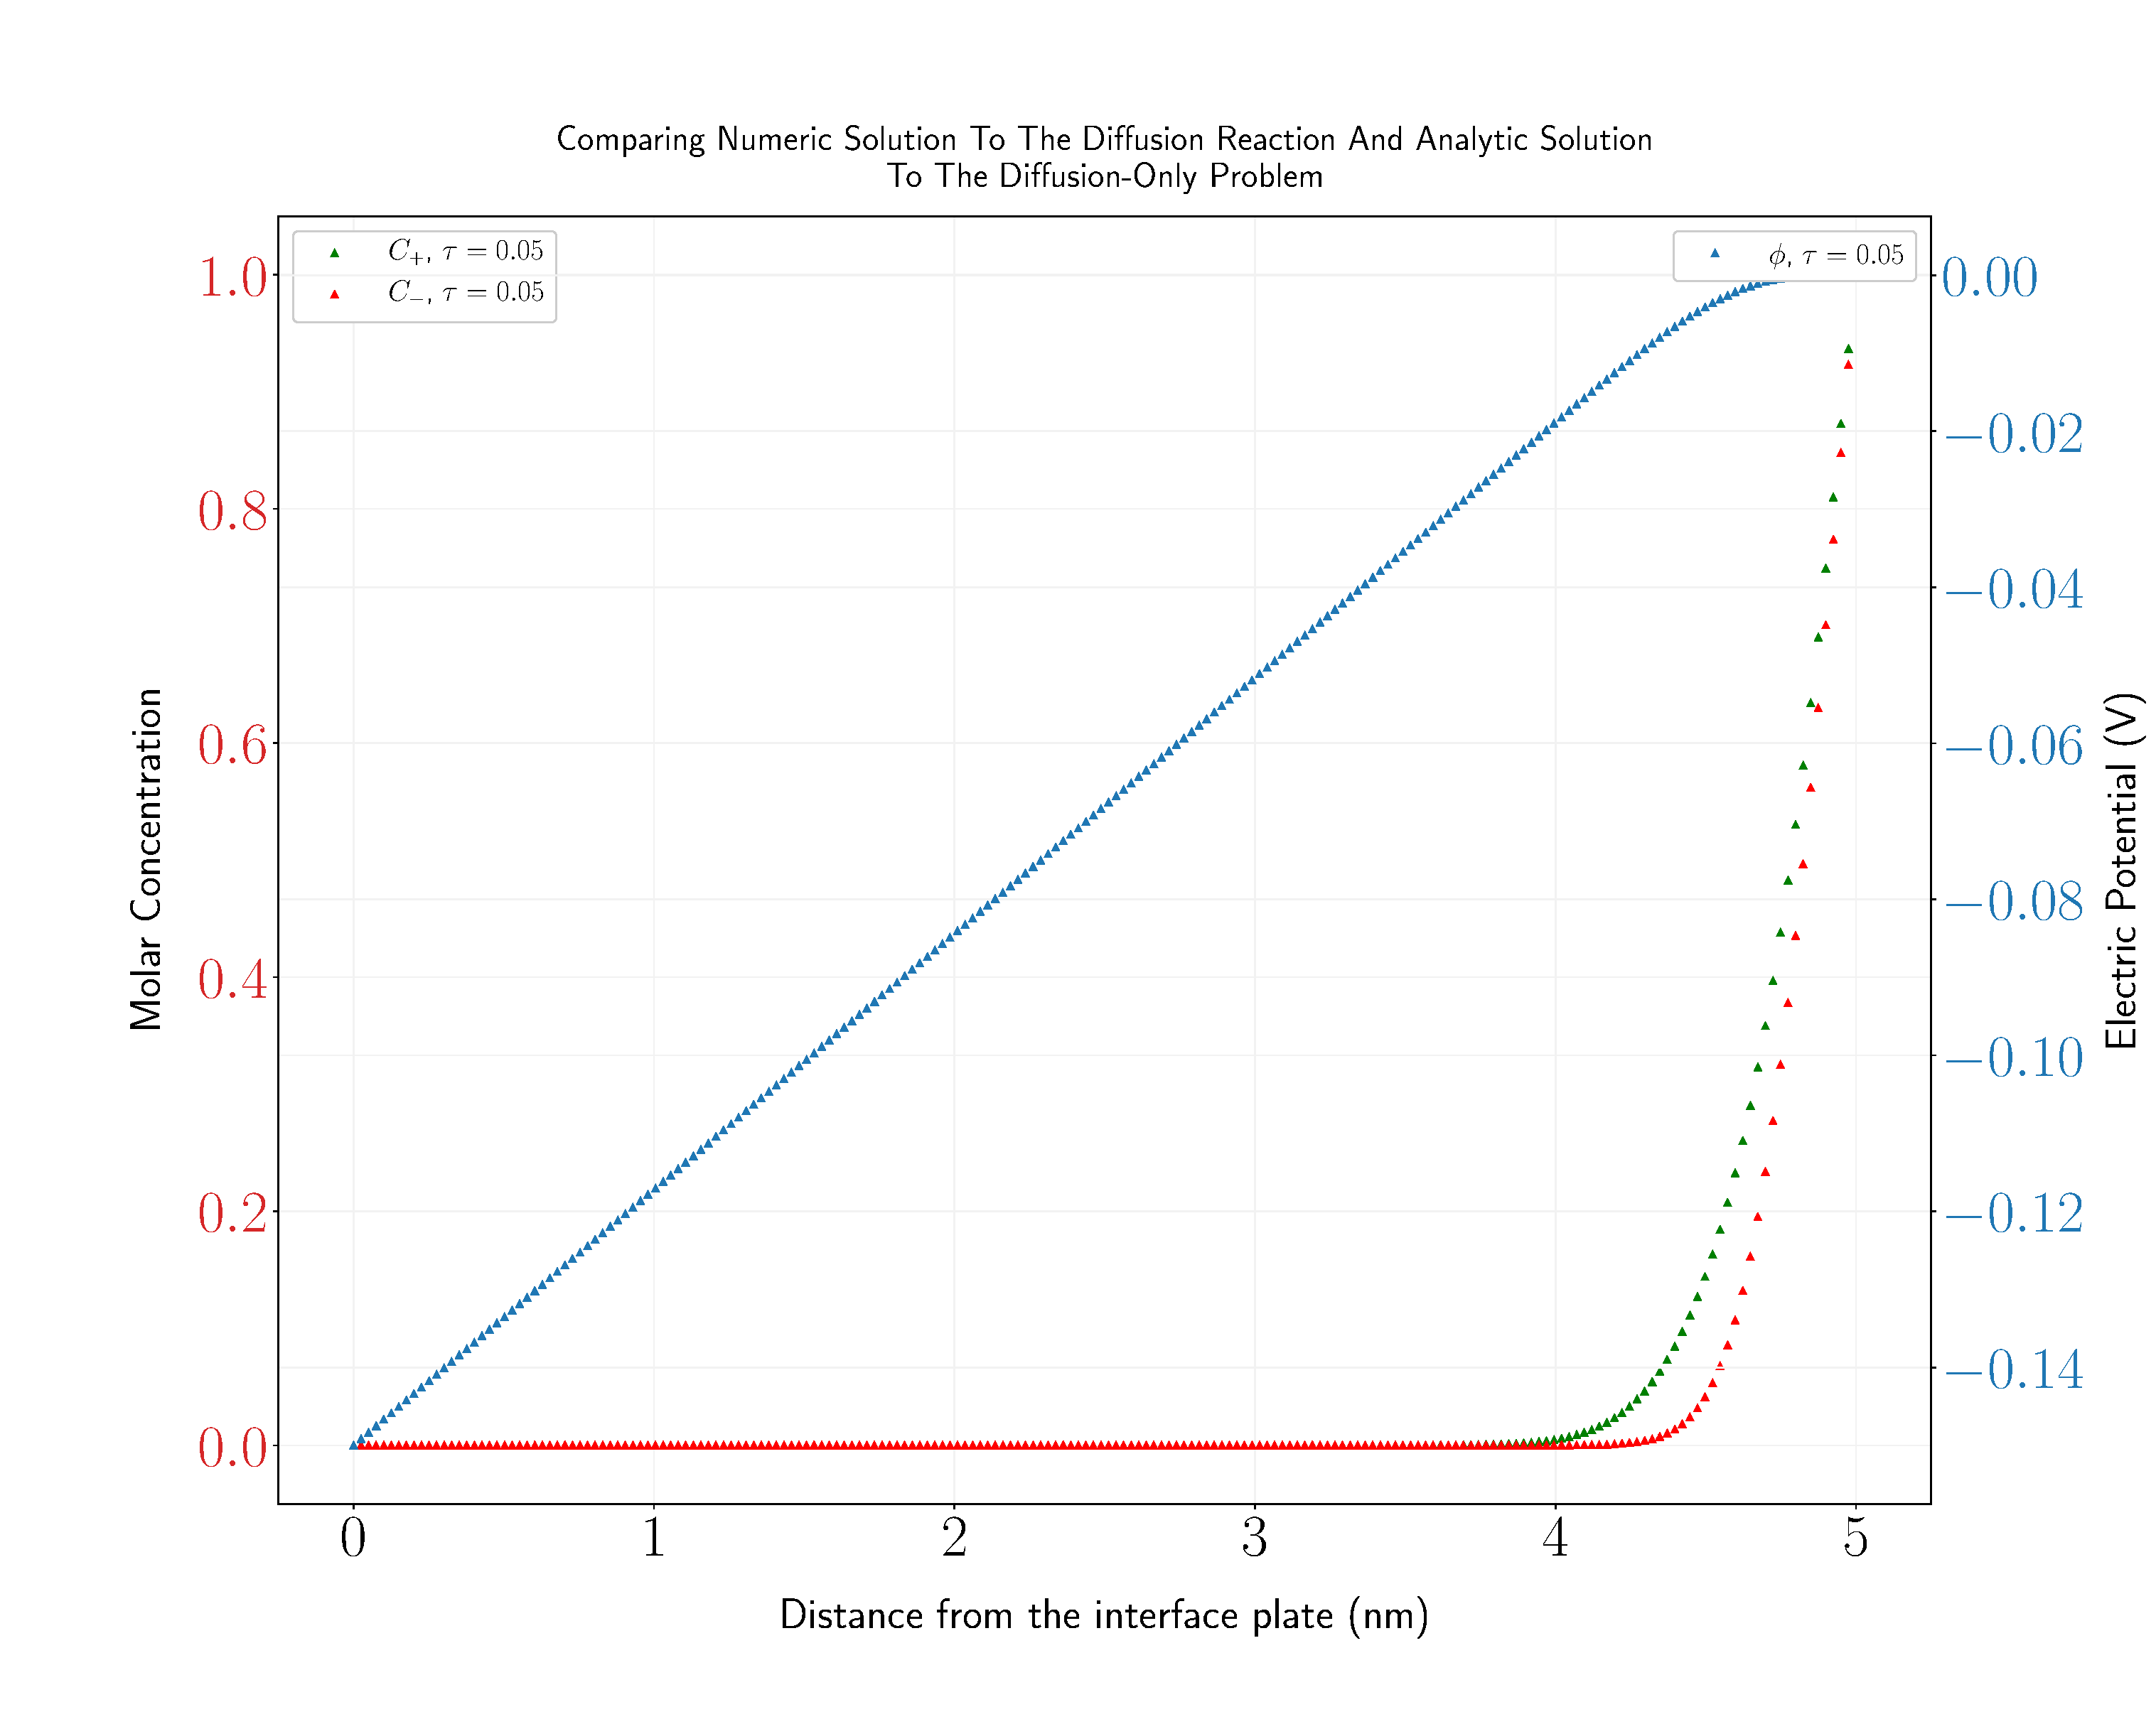
\includegraphics[width=\textwidth]{complete-diffusion-nernst.eps}
\caption{Numerical solution to system \ref{eq:diffusion-nernst}. Red and green dots represent the negative ($SO_4^{-2}$ and positive $Cu^{+2}$ electrolyte concentrations respectively (left axis). The blue dots represent the electric potential (right axis).}
\label{fig:nernst-planck}
\end{figure}









